% Unit 10 / Unit 9 — Central Force, Non-Inertial Frames, Rotating Frames
% Pages 147–173

\chapter{Central Force Motion: Energy Diagrams and Orbits}

\section{Energy Diagrams}

Recall:
\begin{align*}
  E &= \tfrac{1}{2}Mv^2 + U(r) \tag{1} \quad \text{-- handy for evaluating } E \\
  E &= \tfrac{1}{2}M\dot{r}^2 + U_\text{eff}(r) \tag{2} \quad \text{-- only depends on a single coordinate ($\theta$ is hidden)}
\end{align*}

\begin{example}[Central Force on Two Non-Interacting Particles]
\begin{itemize}
  \item Relative velocity: $\vect{v}_0 = \dot{\vect{r}} = \dot{\vect{r}}_1 - \dot{\vect{r}}_2 = \dot{\vect{v}}_1 - \dot{\vect{v}}_2$
\end{itemize}

Thus,
\[
  E = \tfrac{1}{2}Mv_0^2 + U(r) = \tfrac{1}{2}M v_0^2
\]
(why? because $v_0 = \dot{r}$ when used in previous derivations).

To find $U_\text{eff}$:
\[
  U_\text{eff} = \frac{L^2}{2Mr^2} + U(r) = \frac{L^2}{2Mr^2}
\]
since $U(r) = 0$.

Thus, by (2):
\[
  E = \tfrac{1}{2}M\dot{r}^2 + \frac{L^2}{2Mr^2} = \tfrac{1}{2}Mv_0^2
\]

Right as $m_1$ and $m_2$ pass: $r = b$, $\dot{r} = 0$ (motion is armogonal). Thus,
\[
  \frac{L}{2Mb^2} = \tfrac{1}{2}v_0^2
\]
\[
  \Rightarrow \quad L = Mbv_0 \qquad \text{(holds for \emph{all} times because $L$ is constant!)}
\]
\[
  \Rightarrow \quad \boxed{U_\text{eff} = \tfrac{1}{2}Mv_0^2 \frac{b^2}{r^2}}
\]

\textbf{Important trick for conserved values:} find a point at which they are easier to compute, then substitute in the resulting expression everywhere!

\[
  \Rightarrow \quad E = KE + U_\text{eff} = \tfrac{1}{2}M\dot{r}^2 + \tfrac{1}{2}Mv_0^2\frac{b^2}{r^2}
\]

\begin{figure}[H]
\begin{center}
\begin{tikzpicture}
\begin{axis}[
  width=0.5\textwidth, height=4.5cm,
  xlabel={$r$}, ylabel={Energy},
  xmin=0.3, xmax=5, ymin=-0.1, ymax=1.8,
  xtick={1}, xticklabels={$b$},
  ytick={1.0}, yticklabels={$E=\tfrac{1}{2}Mv_0^2$},
  axis lines=left, samples=120,
]
  \addplot[thick,blue,domain=0.32:5]{1/(x*x)} node[pos=0.08,right,scale=0.8]{$U_\text{eff}$};
  \addplot[thick,dashed,red,domain=0.3:5]{1.0} node[pos=0.9,above,scale=0.8]{$E_\text{tot}$};
  % KE region shading
  \addplot[fill=green!20, opacity=0.4, domain=1:5] {1.0} \closedcycle;
\end{axis}
\end{tikzpicture}
\end{center}
\caption{Energy diagram for two non-interacting particles. The effective potential $U_\text{eff} = \frac{1}{2}Mv_0^2 b^2/r^2$ (blue) diverges at $r=0$. The total energy $E = \frac{1}{2}Mv_0^2$ (red dashed) is constant. The kinetic energy $KE = E - U_\text{eff}$ is non-negative; motion is restricted to $r \geq b$.}
\label{fig:eff_pot_centrifugal}
\end{figure}

Since $KE \geq 0$, $E - U_\text{eff} \geq 0$.

This whole setup is equivalent to a single particle $M$ in 1D, $\mu$, moving in $r$-space.
\end{example}

\section{Energy Diagrams and Planetary Motion}

In the context of planetary motion,
\[
  f(r) = -\frac{Gm_1 m_2}{r^2}
\]
\[
  U(\infty) - U(r) = -\int_r^\infty f(r')\,dr' = -\frac{Gm_1 m_2}{r}
\]
Thus,
\[
  U(r) = -\frac{Gm_1 m_2}{r}
\]

Thus,
\[
  U_\text{eff} = \underbrace{\frac{L^2}{2Mr^2}}_{\text{dominates at small }r} - \underbrace{\frac{Gm_1 m_2}{r}}_{\text{dominates at large }r}
\]

Thus,
\[
  E = \tfrac{1}{2}M\dot{r}^2 + \frac{L^2}{2Mr^2} - \frac{Gm_1 m_2}{r}
\]

\begin{figure}[H]
\begin{center}
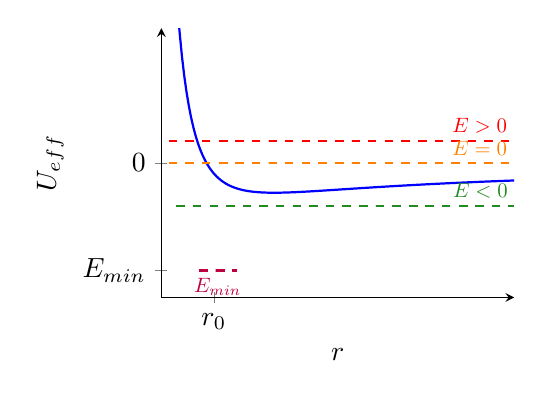
\begin{tikzpicture}
\begin{axis}[
  width=0.5\textwidth, height=5cm,
  xlabel={$r$}, ylabel={$U_\text{eff}$},
  xmin=0.3, xmax=5, ymin=-2.5, ymax=2.5,
  xtick={1.0}, xticklabels={$r_0$},
  ytick={-2.0,0}, yticklabels={$E_\text{min}$,$0$},
  axis lines=left, samples=150,
]
  % Effective potential: L^2/(2mr^2) - C/r
  \addplot[thick,blue,domain=0.42:5]{1.8/(x*x) - 2.0/x} node[pos=0.05,right,scale=0.75]{$U_\text{eff}$};
  % Horizontal energy lines
  \addplot[thick,dashed,red,domain=0.4:5]{0.4}    node[pos=0.9,above,scale=0.75]{$E>0$};
  \addplot[thick,dashed,orange,domain=0.4:5]{0.0} node[pos=0.9,above,scale=0.75]{$E=0$};
  \addplot[thick,dashed,ForestGreen,domain=0.5:5]{-0.8} node[pos=0.9,above,scale=0.75]{$E<0$};
  \addplot[thick,dashed,purple,domain=0.8:1.3]{-2.0} node[pos=0.5,below,scale=0.75]{$E_\text{min}$};
\end{axis}
\end{tikzpicture}
\end{center}
\caption{Effective potential for planetary motion $U_\text{eff}(r) = L^2/(2Mr^2) - C/r$ (blue). Four energy cases: $E>0$ (unbound, hyperbola), $E=0$ (parabola), $E<0$ (bound ellipse), and $E=E_\text{min}$ at $r=r_0$ (circular orbit).}
\label{fig:planetary_eff_pot}
\end{figure}

(See lecture notes for cases.)

\section{Perturbed Circular Orbit}

A satellite of mass $m$ orbits Earth at radius $r_0$ (changes energy of the satellite but not angular momentum) — fires thruster towards the Earth.

\[
  \frac{m_1 m_2}{m_1 + m_2} \approx \frac{m_1 m_e}{m_e} = m_1
\]

\textbf{Approximate solution:} approximate $U_\text{eff}(r)$ in the neighbourhood of $r_0$.

We know $U_\text{eff} = -\frac{C}{r} + \frac{L^2}{2mr^2}$ (since $\mu \approx m$).

\[
  \left.\frac{\partial U_\text{eff}}{\partial r}\right|_{r_0} = \frac{C}{r_0^2} - \frac{L^2}{mr_0^3} = 0
\]
\[
  \Rightarrow \quad L = \sqrt{mCr_0} \qquad (\text{where } C = GmM_E)
\]

We know
\[
  \beta = \sqrt{\frac{k}{m}} = \sqrt{\frac{\partial^2 U_\text{eff}}{\partial r^2}\cdot\frac{1}{m}} \approx \sqrt{\frac{C}{mr_0^3}} = \frac{L}{mr_0^2}
\]

Thus,
\[
  r = r_0 + A\sin(\beta t) + B\cos(\beta t)
\]
Since $r(0) = r_0$:
\[
  r = r_0 + A\sin(\beta t)
\]

\textbf{Finding the new orbit:}
\[
  \dot{\theta} = \frac{L}{mr_0^2} \quad \Rightarrow \quad \theta = \left(\frac{L}{mr_0^2}\right)t \equiv \beta t
\]

Thus,
\[
  r = r_0 + A\sin(\theta)
\]

\chapter{Planetary Motion}

\section{Planetary Motion}

\textbf{Goal:} find the orbital trajectory of a planet of mass $m$ moving about a star of mass $M$ under the gravitational interaction
\[
  U(r) = -G\frac{Mm}{r} = -\frac{C}{r}
\]

Most commonly, $C = GmM_E = mg R_E^2$ for a satellite orbiting the Earth.

Using the $\theta(r)$ equation with $U(r)$:
\[
  \boxed{\theta - \theta_0 = L\int_r \frac{dr}{\sqrt{2MEr^2 + 2MCr - L^2}}}
\]

We can solve the integral to show that
\begin{equation}
  r = \frac{L^2/MC}{1 - \sqrt{1 + (2EL^2/MC^2)}\,\sin(\theta - \theta_0)} \tag{1}
\end{equation}

where $\theta_0$ is conventionally $-\pi/2$ (why?), and
\[
  r_0 = \frac{L^2}{MC} \quad \text{(radius of circular orbit corresponding to $L$, $M$, $C$)}
\]

\begin{formula}[Eccentricity]
\[
  \epsilon \equiv \sqrt{1 + \frac{2EL^2}{MC^2}} \tag{2}
\]
called the \emph{eccentricity}.
\end{formula}

Thus, (1) becomes
\[
  r = \frac{r_0}{1 - \epsilon\cos\theta}
\]

Rewriting in Cartesian coordinates: $r = \sqrt{x^2 + y^2}$, $r\cos\theta = x$,
\begin{align*}
  &\Rightarrow \quad r - \epsilon r\cos\theta = r_0 \\
  &\Rightarrow \quad \sqrt{x^2+y^2} - \epsilon x = r_0
\end{align*}

Squaring:
\[
  r_0^2 = x^2 + y^2 - 2\sqrt{x^2+y^2}\,\epsilon x + \epsilon^2 x^2
\]
\begin{equation}
  \boxed{= (1-\epsilon^2)x^2 - 2r_0\,\epsilon\, x + y^2} \tag{3}
\end{equation}

$\Rightarrow$ is a conic section.

\section{Implications of Eccentricity}

\begin{enumerate}
  \item If $\epsilon > 1$, $E > 0$ (by (2)) $\Rightarrow$ system is unbounded, so has equation of a \textbf{hyperbola}.

  \item $\epsilon = 1 \Rightarrow E = 0$; system is on the border between bounded and unbounded.

  Thus (3) becomes
  \[
    x = \frac{y^2}{2r_0} - \frac{r_0}{2} \quad \Rightarrow \text{ equation of a \textbf{parabola}.}
  \]

  \item $0 \leq \epsilon < 1 \Rightarrow -\frac{MC^2}{2L^2} \leq E < 0$

  $\Rightarrow$ system is bounded, so the equation is of an \textbf{ellipse}.

  (If $E = -\frac{MC^2}{2L^2}$, eq.\ becomes $x^2 + y^2 = r_0^2$, eq.\ of a \textbf{circle}.)
\end{enumerate}

\section{Hyperbolic Orbits}

Examine a projectile $\mu$ with velocity $v_0$, being gravitationally attracted to the atom with \emph{impact parameter} $b$:

\begin{figure}[H]
  \centering
  \caption{Hyperbolic orbit diagram: incoming projectile $\mu$ with velocity $v_0$ and impact parameter $b$, deflected through scattering angle $\psi = \pi - 2\theta_a$. The closest approach is $r_\text{min}$.}
\end{figure}

Thus, we have:
\[
  L = \mu v_0 b \quad \text{(because $\vec{b}$ is $\perp$ to $v_0$)}
\]
\[
  E = \tfrac{1}{2}\mu v_0^2, \qquad U(r) = -C/r
\]
\[
  r = \frac{r_0}{1 - \epsilon\cos\theta} \tag{2}
\]

where
\begin{equation}
  r_0 = \frac{L^2}{MC} = \frac{\mu v_0^2 b^2}{C} = \frac{2Eb^2}{C} \tag{1}
\end{equation}

and
\[
  \epsilon = \sqrt{1 + \frac{2EL^2}{MC^2}} = \sqrt{1 + \left(\frac{2Eb}{C}\right)^2}
\]

Thus, by (1), $L^2 = 2\mu E b^2$.

When $\theta = \pi$, $r = r_\text{min}$, and by (2):
\[
  r_\text{min} = \frac{r_0}{1+\epsilon} = \frac{2Eb^2/C}{1 + \sqrt{1+(2Eb/C)^2}}
\]

Thus, as $E \to \infty$, $r_\text{min} \to b$ $\Rightarrow$ $0 < r_\text{min} < b$.

The half-angle $\theta_a$ between asymptotes, by (2), is found by letting $r \to \infty$:
\begin{equation}
  \cos(\theta_a) = \frac{1}{\epsilon} \tag{3}
\end{equation}

\subsection{Scattering Angle}

The \emph{scattering angle}: the angle that $\mu$ is deflected by ($\psi = \pi - 2\theta_a$).

Thus,
\[
  \cos(\theta_a) = \cos(\pi/2 - \psi/2) = \sin(\psi/2)
\]

So
\[
  \sin(\psi/2) = \frac{1}{\epsilon} = \frac{1}{\sqrt{1 + (2Eb/C)^2}}
\]

\section{Elliptical Orbits and Planetary Motion}

Recall that for $0 \leq \epsilon < 1$:
\[
  (1-\epsilon^2)x^2 - 2r_0\,\epsilon\, x + y^2 = r_0^2
\]

A focus of the ellipse is at the origin (the Sun).

\[
  r_\text{min} + r_\text{max} = A \quad \text{(Major axis)}
  = r_0\!\left(\frac{1}{1+\epsilon} + \frac{1}{1-\epsilon}\right)
  = \frac{2r_0}{1-\epsilon^2}
  = \frac{2L^2/\mu C}{1-(1+2EL^2/\mu C^2)}
\]
\[
  = \underbrace{\frac{C}{-E}}_{\text{independent of }L!}
\]

Thus,
\[
  E = \frac{-C}{A} = \tfrac{1}{2}\mu v_0^2 - \frac{C}{r}
\]

\begin{formula}[Vis-viva equation]
\[
  \boxed{v^2 = \frac{2C}{\mu}\!\left(\frac{1}{r} - \frac{1}{A}\right)}
\]
\emph{Orbital speed at any position $r$.}
\end{formula}

\section{Period of an Elliptic Orbit}

Recall the $r(t)$ equation:
\[
  t_b - t_a = \mu\int_{r_a}^{r_b} \frac{r\,dr}{\sqrt{2\mu Er^2 + 2\mu Cr - L^2}}
\]
(with $E < 0$). Integrating, we find that
\[
  t_b - t_a = \left.\frac{\sqrt{2\mu Er^2 + 2\mu Cr - L^2}}{2E}\right|_{r_a}^{r_b}
\]

Skipping to the result,
\[
  T = \left(\frac{\pi\mu C}{-E}\right)\frac{1}{\sqrt{-2\mu E}}
\]
\[
  T^2 = \frac{\pi^2\mu C^2}{-2E^3} = \frac{\pi^2\mu}{2C}\,A^3 \qquad \leftarrow \text{constant}
\]

\begin{formula}[Kepler's Third Law]
\[
  \boxed{T^2 \propto A^3}
\]
where $k$ is the constant of proportionality — $k$ is about the same for all planets in our solar system!
\end{formula}

\subsection{Simpler Way to Calculate Period}

\[
  L = \mu r^2 \dv{\theta}{t} \quad \Rightarrow \quad \frac{L}{2\mu}\,dt = \tfrac{1}{2}r^2\,d\theta = \text{area element in polar coordinates}
\]

\begin{figure}[H]
  \centering
  \caption{Area swept by the radius vector: the infinitesimal area element $\frac{1}{2}r^2\,d\theta$ in polar coordinates, and the ellipse with semi-axes $b$ and $r_a$.}
\end{figure}

Thus,
\[
  \frac{LT}{2\mu} = \text{area of the ellipse} = \pi ab
\]

where
\[
  a = \frac{A}{2} = \frac{C}{-2E}, \qquad b = \frac{L}{\sqrt{-2\mu E}}
\]

Thus,
\[
  T^2 = \frac{\pi^2\mu}{2C}\,A^3
\]

\section{Orbit Eccentricities}

\begin{itemize}
  \item As $\epsilon \to 0$, $\dfrac{r_\text{max}}{r_\text{min}} \to 1$ $\Rightarrow$ ellipse is roughly circular.
  \item As $\epsilon \to 1$, ellipse gets very elongated.
\end{itemize}

\begin{example}[Geostationary Orbit]
A satellite is \underline{geostationary} if its orbit is in the equatorial plane and its angular velocity $\Omega_e = $ Earth's rotation.

For satellite of mass $m$, $A = 2r$, $\mu \approx m$:
\[
  C = mgR_E^2, \qquad v = r\Omega_e
\]
\[
  v^2 = (r\Omega_e)^2 = \frac{2C}{m}\!\left(\frac{1}{r} - \frac{1}{2r}\right) = \frac{C}{rm}
\]
\[
  r^3 = \frac{gR_E^2}{\Omega_e^2}
\]
\[
  \Rightarrow \quad r = \sqrt[3]{\frac{gR_E^2}{\Omega_e^2}}
\]
\end{example}

\chapter{Non-Inertial Systems and Fictitious Forces}

\section{Non-Inertial Frames}

$\vec{F} = m\vec{a}$ holds \emph{only} for inertial frames (non-accelerating frame).

\begin{figure}[H]
  \centering
  \caption{Three observers Alice, Bob, and Charlie, each moving at different constant velocities $\vec{v}_1$, $\vec{v}_2$. In inertial frames: Charlie sees Alice at $\vec{v}_1$ and Bob at $\vec{v}_2$; Bob sees Alice at $\vec{v}_1 - \vec{v}_2$ and Charlie at $-\vec{v}_2$; Alice sees Bob at $\vec{v}_2 - \vec{v}_1$ and Charlie at $-\vec{v}_1$. $F = ma$ remains unchanged in these inertial frames.}
\end{figure}

What happens in an accelerating frame?

\section{Accelerating Frame}

If Alice is accelerating:
\[
  \vec{a}_\text{Charlie} = \vec{a}_\text{Alice} + \vec{A} \quad \text{(additional acceleration)}
\]
($\vec{a}_\text{rest}$ = acceleration of Alice according to Charlie)

\[
  \vec{a}_\text{Alice} = \vec{a}_\text{Charlie} - \vec{A}
\]
\[
  a' = a - A
\]
\[
  F_\text{Alice} = ma' = m(\vec{a} - \vec{A}) = \vec{F}_\text{rest} - mA
\]

\begin{figure}[H]
  \centering
  \caption{Left (Lab frame): pendulum of mass $m$ with tension $T$ at angle $\theta$, with gravity $mg$ downward and acceleration $\vec{A}$ of the car. Right (Accelerating frame): same pendulum with fictitious force $F_\text{fict} = mA$ pointing backward, gravity $mg$ downward.}
\end{figure}

\textbf{Lab frame equations:}
\begin{align*}
  &\text{(1)}\quad T\cos\theta - mg = 0 \\
  &\text{(2)}\quad T\sin\theta = mA \\
  &T^2\cos^2\theta + T^2\sin^2\theta = (mg)^2 + (mA)^2 \\
  &\Rightarrow \quad T = m\sqrt{g^2 + A^2}
\end{align*}

\textbf{Accelerating frame equations:}
\begin{align*}
  &T\cos\theta - mg = 0 \\
  &T\sin\theta - F_\text{fict} = 0, \quad F_\text{fict} = mA \\
  &\tan\theta = \frac{F_\text{fict}}{mg} \\
  &T = m\sqrt{g^2+A^2}
\end{align*}

$\Rightarrow$ Physical quantities stay the same regardless of which frame we are in.

\subsection{Pendulum in an Accelerating Frame}

What happens when the pendulum starts to oscillate?

\begin{figure}[H]
  \centering
  \caption{Pendulum oscillating in an accelerating car: the new equilibrium point is displaced; the apparent vertical is tilted. In the accelerating frame, apparent gravity $g'$ points at angle $\phi_0$ (combining $mg$ downward and fictitious force $mA$ backward).}
\end{figure}

\begin{itemize}
  \item Apparent gravity is at an angle $\phi_0$.
  \item The tension is also different: $T = m\sqrt{g^2 + A^2}$.
\end{itemize}

\begin{formula}[Pendulum frequency in accelerating frame]
\[
  \boxed{\omega^2 = \frac{g'}{l}}
\]
where $g' = \sqrt{g^2+A^2}$ is the effective gravitational acceleration.
\end{formula}

\section{Rotating Frames}

\subsection{Rotational Coordinates}

A rotating frame is an \underline{accelerating frame}.

\subsubsection{Rate of Change of a Rotating Vector}

Consider a vector $\vec{B}$ rotating at rate $\Omega$ about an axis in direction $\hat{n}$.

\begin{itemize}
  \item $\alpha$: angle between $\vec{B}$ and $\vec{\Omega}$
  \item $\vec{B}$ sweeps out a circular path with radius $B\sin\alpha$
\end{itemize}

Assuming the rotation is at constant $\Omega$, the change of vector $\vec{B}$ is:
\[
  \partial\vec{B} = \vec{B}(t+\Delta t) - \vec{B}(t) = B\sin\alpha\,\Omega\,\Delta\theta \approx (B\sin\alpha)\,\Omega\,\Delta t
\]

By the small-angle approximation:
\[
  \Delta B \approx 2B\sin\alpha\,\sin\!\left(\frac{\Omega\Delta t}{2}\right) \approx (B\sin\alpha)\,\Omega\,\Delta t
\]

\[
  \Rightarrow \quad \frac{\partial\vec{B}}{\partial t} = \lim_{\Delta t\to 0}\frac{B\sin\alpha\,\Omega\,\Delta t}{\Delta t} = (B\sin\alpha)\,\Omega
\]

\begin{formula}[Rate of change of a rotating vector]
\[
  \boxed{\frac{\partial\vec{B}}{\partial t} = \vec{\Omega}\times\vec{B}}
\]
Same as $\dv{\vec{r}}{t} = \vec{\omega}\times\vec{r}$ as derived earlier. Holds true for any vector that undergoes rotation around an axis at rate $\hat{n}$.
\end{formula}

\subsection{Derivative of a Rotating Vector}

Now, let's start with a vector $\vec{C}$ moving in a rotating frame. What is the speed of $\vec{C}$?

In the inertial system:
\[
  \vec{C} = C_x\hat{x} + C_y\hat{y} + C_z\hat{z}
\]

In the rotating system:
\[
  \vec{C} = C_x'\hat{x}' + C_y'\hat{y}' + C_z'\hat{z}'
\]

\[
  \frac{\partial\vec{C}}{\partial t} = \frac{\partial C_x^\text{rot}}{\partial t}\hat{x} + \frac{\partial C_y^\text{rot}}{\partial t}\hat{y} + \frac{\partial C_z^\text{rot}}{\partial t}\hat{z}
  + C_x\frac{\partial\hat{x}}{\partial t} + C_y\frac{\partial\hat{y}}{\partial t} + C_z\frac{\partial\hat{z}}{\partial t}
\]

Given that $\dfrac{\partial\hat{x}}{\partial t} = \vec{\Omega}\times\hat{x}$ (due to rotating in a rotating frame!),

\begin{formula}[Time derivative in rotating frame]
\[
  \frac{\partial\vec{C}}{\partial t} = \left(\frac{\partial\vec{C}}{\partial t}\right)^\text{in frame} + \vec{\Omega}\times\vec{C}
\]
\end{formula}

The non-inertial terms are:
\[
  C_x(\vec{\Omega}\times\hat{x}') + C_y(\vec{\Omega}\times\hat{y}') + C_z(\vec{\Omega}\times\hat{z}') = \vec{\Omega}\times(C_x'\hat{x}' + C_y'\hat{y}' + C_z'\hat{z}') = \vec{\Omega}\times\vec{C}
\]

Think of it as an operator:
\[
  \left(\frac{d}{dt}\right)_\text{in} = \left(\frac{d}{dt}\right)_\text{rot} + \vec{\Omega}\times
\]

\section{Velocity and Acceleration in a Rotating Frame}

For position, we have:
\[
  \left(\frac{\partial\vec{r}}{\partial t}\right)_\text{in} = \left(\frac{\partial\vec{r}}{\partial t}\right)_\text{rot} + \vec{\Omega}\times\vec{r}
\]
\[
  \Rightarrow \quad \vec{v}_\text{in} = \vec{v}_\text{rot} + \vec{\Omega}\times\vec{r}
\]

Taking the derivative of this expression:
\[
  \vec{a}_\text{in} = \vec{a}_\text{rot} + 2\vec{\Omega}\times\vec{v}_\text{rot} + \vec{\Omega}\times(\vec{\Omega}\times\vec{r})
\]

The full derivation:
\[
  \left(\frac{\partial\vec{v}_\text{in}}{\partial t}\right)_\text{in}
  = \left[\frac{\partial}{\partial t}\!\left(\vec{v}_\text{rot} + \vec{\Omega}\times\vec{r}\right)\right]_\text{rot} + \vec{\Omega}\times\!\left(\vec{v}_\text{rot} + \vec{\Omega}\times\vec{r}\right)
\]
\[
  = \left(\frac{\partial\vec{v}_\text{rot}}{\partial t}\right)_\text{rot} + \vec{\Omega}\times\!\left(\frac{\partial\vec{r}}{\partial t}\right) + \vec{\Omega}\times\!\left(\vec{v}_\text{rot} + \vec{\Omega}\times\vec{r}\right)
\]
\[
  \frac{\partial\vec{v}_\text{in}}{\partial t} = \left(\frac{\partial\vec{v}_\text{rot}}{\partial t}\right)_\text{rot} + 2\vec{\Omega}\times\vec{v}_\text{rot} + \vec{\Omega}\times(\vec{\Omega}\times\vec{r})
\]

\begin{formula}[Acceleration in terms of frames]
\[
  \boxed{\underbrace{\vec{a}_\text{in}}_{\text{inertial frame}} = \vec{a}_\text{rot} + 2\vec{\Omega}\times\vec{v}_\text{rot} + \vec{\Omega}\times\!\left(\vec{\Omega}\times\vec{r}\right)}
\]
\end{formula}

\section{Fictitious Forces in a Rotating Coordinate System}

In the rotating frame, $\vec{F}_\text{rot} = m\vec{a}_\text{rot}$:

\begin{formula}[Fictitious forces in rotating frame]
\[
  \vec{F}_\text{rot} = m\vec{a}_\text{in} - \underbrace{2m\vec{\Omega}\times\vec{v}_\text{rot}}_{\text{Coriolis force}} - \underbrace{m\vec{\Omega}\times(\vec{\Omega}\times\vec{r})}_{\text{Centrifugal force}}
\]
\end{formula}

Let $\vec{\Omega} = \Omega\hat{z}$. In spherical coordinates ($\hat{z}$, $\hat{r}$, $\hat{\theta}$):
\[
  \vec{\Omega} = \Omega\hat{z}
\]
\[
  \vec{r} = r\sin\alpha\,\hat{\rho} + r\cos\alpha\,\hat{z}
\]
\[
  \vec{\Omega}\times\vec{r} = \Omega\,r\sin\alpha\,(\hat{z}\times\hat{\rho}) = \Omega\,r\sin\alpha\,\hat{\theta}
\]

\[
  \vec{\Omega}\times(\vec{\Omega}\times\vec{r}) = \vec{\Omega}\times(\Omega\,r\sin\alpha\,\hat{\theta})
  = \Omega^2 r\sin\alpha\,(\hat{z}\times\hat{\theta})
  = -\Omega^2 r\sin\alpha\,\hat{\rho}
\]

\begin{example}[Falling Object in a Rotating Frame]
\begin{figure}[H]
  \centering
  \caption{A mass $m$ falling near the surface of the rotating Earth (depicted as a circle with rotation $\Omega$).}
\end{figure}
\end{example}

\chapter{Non-Inertial Systems: Rotating Coordinates (9.1--9.5)}

\section{Rate of Change of a Rotating Vector}

\begin{itemize}
  \item Consider a vector $\vec{B}$ that is rotating at rate $\Omega$ about an axis in direction $\hat{n}$.
  \item $\alpha$: angle between $\vec{B}$ and $\vec{\Omega}$.
  \item $\vec{B}$ sweeps out a circular path with radius $B\sin\alpha$.
\end{itemize}

By the small-angle approximation:
\[
  \Delta B = 2B\sin\alpha\,\sin\!\left(\frac{\Omega\Delta t}{2}\right) \approx (B\sin\alpha)\,\Omega\,\Delta t
\]

\[
  \Rightarrow \quad \frac{\partial\vec{B}}{\partial t} = \lim_{\Delta t\to 0}\frac{B\sin\alpha\,\Omega\,\Delta t}{\Delta t} = (B\sin\alpha)\,\Omega = \vec{\Omega}\times\vec{B} = \frac{\partial\vec{B}}{\partial t}
\]

Holds true for any vector that undergoes rotation around an axis at rate $\hat{n}$.

\section{Time Derivative of a Vector in a Rotating Coordinate System}

Consider any vector $\vec{C}$ changing at rate $\left(\dfrac{\partial\vec{C}}{\partial t}\right)_\text{in}$ as observed in an inertial system. (We are not rotating.)

Problem: find the time derivative $\left(\dfrac{\partial\vec{C}}{\partial t}\right)_\text{rot}$ in a rotating coordinate system.

In the inertial system:
\[
  \vec{C} = C_x\hat{i} + C_y\hat{j} + C_z\hat{k}
\]

In the rotating system:
\[
  \vec{C} = C_x'\hat{i}' + C_y'\hat{j}' + C_z'\hat{k}'
\]

But by the previous result:
\[
  \frac{\partial\hat{i}'}{\partial t} = \vec{\Omega}\times\hat{i}', \quad
  \frac{\partial\hat{j}'}{\partial t} = \vec{\Omega}\times\hat{j}', \quad
  \frac{\partial\hat{k}'}{\partial t} = \vec{\Omega}\times\hat{k}' \qquad \text{(Non-inertial terms)}
\]

Thus,
\[
  \left(\frac{\partial\vec{C}}{\partial t}\right)_\text{rot} = \left(\frac{\partial C_x'}{\partial t}\hat{i}' + \frac{\partial C_y'}{\partial t}\hat{j}' + \frac{\partial C_z'}{\partial t}\hat{k}'\right)
  + \left(C_x'\frac{\partial\hat{i}'}{\partial t} + C_y'\frac{\partial\hat{j}'}{\partial t} + C_z'\frac{\partial\hat{k}'}{\partial t}\right)
\]

The second bracket equals:
\[
  C_x'(\vec{\Omega}\times\hat{i}') + C_y'(\vec{\Omega}\times\hat{j}') + C_z'(\vec{\Omega}\times\hat{k}') = \vec{\Omega}\times(C_x'\hat{i}' + C_y'\hat{j}' + C_z'\hat{k}') = \vec{\Omega}\times\vec{C}
\]

\[
  \Rightarrow \quad \boxed{\left(\frac{\partial\vec{C}}{\partial t}\right)_\text{in} = \left(\frac{\partial\vec{C}}{\partial t}\right)_\text{rot} + \vec{\Omega}\times\vec{C}}
\]

Think of it as an operator:
\[
  \left(\frac{d}{dt}\right)_\text{in} = \left(\frac{d}{dt}\right)_\text{rot} + \vec{\Omega}\times
\]

\section{Velocity and Acceleration in a Rotating Coordinate System}

For position, we have:
\[
  \left(\frac{\partial\vec{r}}{\partial t}\right)_\text{in} = \left(\frac{\partial\vec{r}}{\partial t}\right)_\text{rot} + \vec{\Omega}\times\vec{r}
\]
\[
  \Rightarrow \quad \vec{v}_\text{in} = \vec{v}_\text{rot} + \vec{\Omega}\times\vec{r}
\]

Taking the derivative of this expression:
\[
  \vec{a}_\text{in} = \vec{a}_\text{rot} + 2\vec{\Omega}\times\vec{v}_\text{rot} + \vec{\Omega}\times(\vec{\Omega}\times\vec{r})
\]

\subsection{Fictitious Forces}

Thus, $m\vec{a}_\text{in} = \vec{F}_m$:
\[
  \vec{F}_\text{rot} = \vec{F}_\text{in} - \underbrace{2m\vec{\Omega}\times\vec{v}_\text{rot}}_{\text{Coriolis}} - \underbrace{m\vec{\Omega}\times(\vec{\Omega}\times\vec{r})}_{\substack{\text{Centrifugal}\\F_c = -m\vec{\Omega}\times(\vec{\Omega}\times\vec{r})}}
\]

\begin{itemize}
  \item Centrifugal force magnitude: $m\Omega^2\rho$ (where $\rho$ is the perpendicular distance from the axis of rotation to the tip of $\vec{r}$).
  \item Coriolis: fictitious force to balance the Coriolis acceleration $2\vec{\Omega}\times\vec{v}_\text{rot}$.
  \item Coriolis magnitude: $2m\dot{r}\omega$ (for $v_\rho$) or $2mr\dot{\theta}\omega$ (for $v_\theta$).
\end{itemize}

\textbf{Important:} $\vec{v}_\text{rot}$ is velocity in the \emph{rotating} frame, not the inertial frame!

\begin{fact}[Horizontal Coriolis force]
\[
  \vec{F}_H = -2m\Omega\sin\lambda\,(\hat{r}\times\vec{v}) \qquad \text{(horizontal component)}
\]
\end{fact}

\begin{example}[Surface of a Rotating Liquid]
\begin{figure}[H]
  \centering
  \caption{Rotating liquid bucket: in the rotating frame, forces on a fluid element are normal force $F_\text{norm}$, centrifugal force $m\omega^2 r$ outward, and gravity $W = mg$ downward. The surface tilts so that $\phi = \tan^{-1}(\omega^2 r / g)$.}
\end{figure}

Equations of equilibrium in the rotating frame:
\[
  F_0\cos\phi - W = 0
\]
\[
  -F_0\sin\phi + F_\text{cent} = 0
\]
\[
  \Rightarrow \quad F_\text{cent} = m\Omega^2 r = m\omega^2 r \quad (\text{since } \Omega = \omega \text{ for a coordinate system with rotating bucket})
\]

\begin{formula}[Shape of rotating liquid surface]
\[
  \phi = \tan^{-1}\!\left(\frac{\omega^2 r}{g}\right) \qquad \text{important tool!}
\]
\[
  \boxed{\frac{dz}{dr} = \tan\phi = \frac{\omega^2 r}{g}}
\]
\end{formula}

Integrating:
\[
  \int dz = \frac{\omega^2}{g}\int r\,dr = \tfrac{1}{2}\frac{\omega^2}{g}r^2
\]

The surface is a paraboloid $z = \dfrac{\omega^2}{2g}r^2$.
\end{example}

\begin{example}[Sliding Bead and Coriolis Forces]
A bead slides without friction on a horizontal wire. Find the force exerted on the bead by the wire.

\begin{figure}[H]
  \centering
  \caption{Bead on a horizontal rotating wire: in the rotating frame, the bead at distance $r$ experiences centrifugal force $F_\text{cent}$ outward and Coriolis (normal) force $N$ perpendicular to the wire.}
\end{figure}

Equations of motion:
\[
  F_\text{cent} = m\ddot{r}, \qquad N - F_\text{Cor} = 0 \quad \Rightarrow \quad N = F_\text{Cor}
\]
\[
  F_\text{cent} = m\omega^2 r \quad \Rightarrow \quad m\ddot{r} = m\omega^2 r
\]

which has solution $r = Ae^{\omega t} + Be^{-\omega t}$.

(The Coriolis force $F_\text{Cor}$ is found similarly.)
\end{example}

\begin{example}[Deflection of a Falling Mass]

\begin{figure}[H]
  \centering
  \caption{Mass $m$ falling near the rotating Earth (rotation $\Omega$), with motion confined to the equatorial plane. The coordinates $\hat{r}$ (radial) and $\hat{\theta}$ (tangential) are shown.}
\end{figure}

\[
  \vec{F} = -mg\hat{r} - 2m\vec{\Omega}\times\vec{v}_\text{rot} - m\vec{\Omega}\times(\vec{\Omega}\times\vec{r})
\]

Motion is confined to the equatorial plane:
\[
  \vec{v}_\text{rot} = \dot{r}\hat{r} + r\dot{\theta}\hat{\theta}
\]
\[
  \vec{\Omega}\times\vec{v}_\text{rot} = \Omega\dot{r}\hat{\theta} - r\Omega\dot{\theta}\hat{r}, \qquad \vec{\Omega}\times(\vec{\Omega}\times\vec{r}) = \Omega^2 r\hat{r}
\]

\textit{Tip: this doesn't change that the $\hat{r}$, $\hat{\theta}$ equations of motion still apply.}

\[
  \vec{F}_\text{rot} = -mg\hat{r} - 2m(\Omega\dot{r}\hat{\theta} - r\Omega\dot{\theta}\hat{r}) - mr\Omega^2\hat{r}
\]
\[
  \vec{F}_\text{rad} = -mg\hat{r} + 2mr\Omega\dot{\theta}\hat{r} - mr\Omega^2\hat{r}
\]
\[
  \vec{F}_\text{tan} = -2m\Omega\dot{r}\hat{\theta} = mr\ddot{\theta}
\]

We can omit terms with $\dot{\theta}$ because $m$ falls approximately vertically:
\[
  \ddot{r} \approx -g + \Omega^2 r
\]
\[
  r\ddot{\theta} \approx -2\dot{r}\Omega
\]

We can also take $r \approx R_E$, and let $g$ be constant:
\[
  \Rightarrow \quad \ddot{r} \approx -g' \quad \text{where } g' = g - \Omega^2 R_E
\]

Thus,
\[
  \dot{r} = -g't, \qquad r = r_0 - \tfrac{1}{2}g't^2
\]

\[
  r\ddot{\theta} = 2g't\Omega \quad \Rightarrow \quad \dot{\theta} = \frac{g't^2\Omega}{R_E}
\]
\[
  \Rightarrow \quad \dot{\theta} = \frac{g\Omega}{R_E}t^2
\]
\[
  \Rightarrow \quad \theta = \frac{1}{2}\frac{g\Omega}{R_E}t^3
\]

Thus, the horizontal deflection of $m$ is:
\[
  y \approx R_E\theta \approx \tfrac{1}{3}g\Omega t^3
\]

Time $T$ to fall a distance $h$ is given by:
\[
  r - r_0 = -h = -\tfrac{1}{2}g't^2 \quad \Rightarrow \quad T = \sqrt{\frac{2h}{g}}
\]
\[
  y = \tfrac{1}{2}g\Omega\!\left(\frac{2h}{g}\right)^{3/2}
\]
\end{example}

\begin{example}[Motion on the Rotating Earth]

\[
  \vec{F}_\text{Cor} = -2m(\vec{\Omega}\times\vec{v})
\]

\begin{figure}[H]
  \centering
  \caption{The rotating Earth with rotation $\vec{\Omega}$, showing decomposition of $\vec{\Omega}$ into vertical ($\Omega_V$) and horizontal ($\Omega_H$) components at latitude $\lambda$.}
\end{figure}

\begin{itemize}
  \item Consider a velocity $\vec{v}$ transverse to the rotation.
  \item Horizontal component of Coriolis force is $\perp$ to $\vec{v}$ and its magnitude is independent of direction of $\vec{v}$.
\end{itemize}

Thus,
\begin{align*}
  \vec{F} &= -2m(\vec{\Omega}\times\vec{v}) \\
  &= -2m(-\Omega_V\times\vec{v} + \Omega_H\times\vec{v}) \\
  &= \vec{F}_V + \vec{F}_H \quad ?
\end{align*}
\end{example}

\chapter{Morin Chapter 2 Problems}

\begin{example}[2.1 --- Hanging Chain Tension]
A chain of uniform linear mass density $\rho$ and length $L$ hangs vertically ($\rho L = m$).

\begin{figure}[H]
  \centering
  \caption{Hanging chain of length $L$: at height $y$ from the bottom, a segment of length $y$ has weight $\rho y g$, requiring tension $T(y)$.}
\end{figure}

At point $y$, it is being held up by tension $T(y)$ and pulled down by gravity $\rho y g$:
\[
  T(y) - \rho y g = 0
\]
\[
  \Rightarrow \quad \boxed{T(y) = \rho g y}
\]
\end{example}

\begin{example}[2.3 --- Motionless Chain]
A chain of linear mass density $\rho$ lies at rest on an inclined plane at angle $\theta$.

\begin{figure}[H]
  \centering
  \caption{Chain element $\Delta\ell$ on an incline: the component of gravity along the slope is $\Delta F = g\sin\theta\,dm$, with $\sin\theta = \Delta y/\sqrt{\Delta x^2+\Delta y^2}$ and $\Delta\ell = \sqrt{\Delta x^2+\Delta y^2}$.}
\end{figure}

\[
  \Delta F = g\sin\theta\cdot dm = g\sin\theta\cdot\rho\,\Delta\ell, \qquad
  \sin\theta = \frac{\Delta y}{\sqrt{\Delta x^2+\Delta y^2}}, \quad \Delta\ell = \sqrt{\Delta x^2+\Delta y^2}
\]

\[
  \Rightarrow \quad \Delta F = g\frac{\Delta y}{\sqrt{\Delta x^2+\Delta y^2}}\cdot\rho\sqrt{\Delta x^2+\Delta y^2}
\]
\[
  \Rightarrow \quad \Delta F = \rho g\,\Delta y
\]

\[
  F = \int dF = \rho g\int_{y_0}^{y_1} dy = \rho g(y_0 - y_1) = 0
\]
\[
  \boxed{F_\text{net} = 0}
\]

(The net gravitational force along the slope is zero for a chain between two points at the same height, regardless of the shape of the path.)
\end{example}

\begin{example}[2.4 --- Minimum Force to Keep a Book Up]
A book of mass $M$ is pushed against a wall with a force $F$ at angle $\theta$, with friction coefficient $\mu$.

\begin{figure}[H]
  \centering
  \caption{Book against wall: applied force $F$ at angle $\theta$, normal force $N$ from wall (horizontal), friction $f$ upward along wall.}
\end{figure}

Equations:
\begin{align*}
  &\text{(1)}\quad F\cos\theta = N \\
  &\text{(2)}\quad F\sin\theta + f = Mg \\
  &\text{(3)}\quad f \leq \mu N
\end{align*}

From (1) and (3): $f \leq \mu F\cos\theta$.

From (2): $F\sin\theta + \mu F\cos\theta \geq Mg$, so $F(\sin\theta + \mu\cos\theta) \geq Mg$:
\[
  \boxed{F \geq \frac{Mg}{\sin\theta + \mu\cos\theta}} \qquad \text{assuming } \sin\theta + \mu\cos\theta > 0
\]

To minimize $F$, set $\dfrac{dF}{d\theta} = 0$:
\[
  \frac{dF}{d\theta} = \frac{-Mg}{(\sin\theta+\mu\cos\theta)^2}(\cos\theta - \mu\sin\theta) = 0
\]
\[
  \cos\theta - \mu\sin\theta = 0 \quad \Rightarrow \quad \boxed{\tan\theta = \frac{1}{\mu}}
\]

\begin{figure}[H]
  \centering
  \caption{Right triangle: opposite side $1$, adjacent side $\mu$, hypotenuse $\sqrt{1+\mu^2}$.}
\end{figure}

\[
  F \geq \frac{Mg}{\dfrac{\cos\theta}{\mu}+\mu\cos\theta} = \frac{Mg\mu}{(1+\mu^2)\cos\theta} = \frac{Mg}{(1+\mu^2)}\cdot\frac{1}{\sin\theta} = \frac{Mg}{\sqrt{1+\mu^2}}
\]

\[
  \boxed{F_\text{min} = \frac{Mg}{\sqrt{1+\mu^2}}}
\]

\textbf{Part (c):} If $\sin\theta = -\mu\cos\theta \Rightarrow \tan\theta = -\mu$:
\[
  \theta = -\tan^{-1}(\mu); \text{ if } \theta < -\tan^{-1}(\mu) \text{ then it is impossible to keep the book up.}
\]
\end{example}

\begin{example}[2.5 --- Rope on a Plane]

\textbf{Case 1:} A rope of linear density $\rho$ lies on an inclined plane at angle $\theta$, with friction coefficient $\mu$. Find the maximum tension distribution.

\begin{figure}[H]
  \centering
  \caption{Element $dm$ of rope on incline: tension $T(x)$ at left end, $T(x+dx)$ at right end, normal force $N$, friction $f$, and component of gravity $\rho\,dx\cdot g\sin\theta$ along the slope.}
\end{figure}

Equations:
\begin{align*}
  &\text{(1)}\quad T(x) + f = \rho\,dx\cdot g\sin\theta + T(x+dx) \\
  &\text{(2)}\quad f \leq \mu N = \mu\,\rho\,dx\,g\cos\theta
\end{align*}

Combining:
\[
  \mu\,\rho\,dx\,g\cos\theta \geq \rho\,dx\,g\sin\theta + T(x+dx) - T(x)
\]
\[
  \rho\,dx\,g(\mu\cos\theta - \sin\theta) \geq T(x+dx) - T(x)
\]
\[
  \frac{dT}{dx} \leq \rho g(\mu\cos\theta - \sin\theta)
\]
\[
  T(x) \leq \rho g x(\mu\cos\theta - \sin\theta)
\]
\end{example}

\section{Galilean Transformation}

Used to transfer between frames going at different velocities (but parallel axes though).

\begin{figure}[H]
  \centering
  \caption{Two frames: frame $A$ with position $\vec{r}_A$ and frame $B$ displaced by $\vec{S}$, with $\vec{r}_B = \vec{r}_A - \vec{S}$.}
\end{figure}

We have that
\begin{equation}
  \vec{r}_B = \vec{r}_A - \vec{S} \tag{1}
\end{equation}

Suppose that the mass accelerates at:
\begin{itemize}
  \item Alice: $\vec{F}_a = m\vec{a}_a$
  \item Bob observes $\vec{F}_B = M\vec{a}_B$ \quad -- are they the same?
\end{itemize}

By differentiating (1), we get:
\[
  \vec{v}_B = \vec{v}_A - \vec{V} \quad \Bigg\} \text{ Galilean transformation}
\]
\[
  \vec{a}_B = \vec{a}_A - \vec{A}
\]

If $S = $ const or $\vec{v} = $ const $\Rightarrow \vec{A} = \vec{0}$:
\[
  \vec{a}_B = \vec{a}_A \quad \Rightarrow \quad \vec{F}_B = \vec{F}_A
\]

\textbf{Assumptions:}
\begin{itemize}
  \item Lengths are measured the same (not true due to special relativity).
  \item Also time is not the same due to $g$.
\end{itemize}

\subsection{Principle of Relativity}

\textbf{Conclusion:} Laws of physics are the same in all inertial reference frames!

\section{Uniformly-Accelerating Systems}

How physics appears to an observer in a system accelerating at a constant rate $A$:
\[
  \vec{a}' = \vec{a} - \vec{A} \qquad (\text{system acceleration})
\]
(acceleration w.r.t. accelerating frame = acceleration to rest frame minus system acceleration)

\textbf{Apparent Force:}
\[
  \vec{F}' = m\vec{a}' = m\vec{a} - m\vec{A} = \vec{F} + \underbrace{\vec{F}_\text{fict}}_{= -m\vec{A}}
\]

\begin{example}[Apparent Force of Gravity]

\begin{figure}[H]
  \centering
  \caption{Pendulum in an accelerating car (acceleration $A$ to the right). Goal: find the motion.}
\end{figure}

\textbf{Laboratory system:}
\begin{align*}
  &T\sin\theta = mA \\
  &T\cos\theta = mg \\
  &\tan\theta = \frac{A}{g} \\
  &T^2 = m^2(A^2+g^2) \\
  &T = m\sqrt{A^2+g^2}
\end{align*}

\textbf{Accelerating system} ($F_\text{net} = ma = 0$):
\begin{align*}
  &T\cos\theta - W = 0 \\
  &T\sin\theta - F_\text{fict} = T\sin\theta - mA = 0 \\
  &\tan\theta = \frac{A}{g} \\
  &\Rightarrow \quad T = m\sqrt{A^2+g^2}
\end{align*}
\end{example}

\begin{example}[Cylinder on an Accelerating Plank]
A cylinder of radius $R$, mass $M$ sits on a plank that accelerates at rate $A$. No slip condition.

\begin{figure}[H]
  \centering
  \caption{Cylinder (radius $R$, mass $M$) on an accelerating plank (acceleration $A$): friction force $f$ acts on the cylinder, and a fictitious force $F_\text{fict} = mA$ acts backward in the accelerating frame.}
\end{figure}

In the accelerating frame:
\[
  f - \vec{F}_\text{fict} = ma', \qquad \text{no slip} \Rightarrow Rf = -I\alpha' = -\frac{Ia'}{R}
\]

Thus, $f = -\dfrac{Ia'}{R^2}$:
\[
  -\frac{Ia'}{R^2} - F_\text{fict} = ma'
\]
\[
  \Rightarrow \quad a' = \frac{F_\text{fict}}{M + \frac{I_0}{R^2}} = -\frac{2}{3}A
\]

Thus,
\[
  a = a' + A = \boxed{\frac{1}{3}A}
\]
\end{example}

\begin{example}[Pendulum in an Accelerating Car]
\begin{figure}[H]
  \centering
  \caption{Pendulum in accelerating car: equilibrium angle shifts to $\phi_0$; the full oscillation amplitude is $\phi = 2\phi_0 = 2J$.}
\end{figure}

Since we already know:
\[
  \phi_0 = \tan^{-1}\!\left(\frac{A}{g}\right), \qquad \phi = 2\phi_0 = 2J
\]
\end{example}

\section{Principle of Equivalence}

\begin{itemize}
  \item Laws of physics are the same in a uniformly accelerating system as long as we add a fictitious force $\vec{F}_\text{fict} = -m\vec{A}$.
  \item $\vec{F}_\text{fict}$ is indistinguishable from the force due to a uniform gravitational field $\vec{g} = -\vec{A}$.
  \item A particle in deep space free of any physical interactions but uniformly accelerating at $\vec{A} = -g$, it experiences fictitious force $\vec{F}_\text{fict} = -m\vec{A} = m\vec{g}$.
\end{itemize}

\begin{example}[Elevator Thought Experiment]

\textbf{Situation 1:} Person in a box on Earth, gravity $g$ downward.

\textbf{Situation 2:} Person in a box in deep space, box accelerating upward at $a = g$.

If the man drops the apple in both situations, they both appear to accelerate downward at rate $g$ relative to the man.

However, one might conclude that they are in a uniform gravitational field throughout all of space --- unphysical thought!

\begin{formula}[Principle of Equivalence]
No way to locally distinguish between a uniform gravitational acceleration $\vec{g}$ and an acceleration of the coordinate system $\vec{A} = -\vec{g}$.

(Locally means from within a sufficiently-defined system) --- to distinguish, you need a third reference point for plausible denial.
\end{formula}
\end{example}

\begin{example}[Driving Force of the Tides]
According to the principle of equivalence, it is impossible to observe the Sun's gravitational force on an Earth-bound system.

However, the Earth is so large it has non-local effects.
\begin{itemize}
  \item Tides due to the Sun and Moon creating an apparent gravitational field.
\end{itemize}

At the Earth's center A:
\[
  \vec{G}_0 = \frac{GM_s}{r_s^2}\hat{n}
\]

Earth accelerates toward the Sun at rate $A = G_0$.

Let $G(r)$ be the gravitational field at some point $r$ on the Earth. Then $\vec{F} = mG(r)$.

To an Earth-bound observer the force $F' = \vec{F} - m\vec{A}$:
\[
  = mG(r) - mG_0
\]

The apparent field is thus:
\[
  \frac{F'}{m} = G'(r) = G(r) - G_0
\]

\begin{figure}[H]
  \centering
  \caption{Left: Sun and Earth with gravitational fields $G_A$, $G_B$, $G_C$, $G_D$, $G_E$ at various points on the Earth (center A, near-side B, far-side C, top D, bottom E), with Earth-Sun distance $r_s$. Right: residual (tidal) fields $G_A' = 0$, $G_B'$ pointing toward Sun, $G_C'$ pointing away, $G_D'$ and $G_E'$ pointing inward (neglecting higher-order terms).}
\end{figure}

\[
  G_A' = G_A - G_0 = \frac{GM_s}{(r_s - R_E)^2} - G_0 \approx 2G_0\frac{R_E}{r_s}
\]

$G_C'$ is similar: $= -2G_0\dfrac{R_E}{r_s}$.

Using small-angle approximation: $G_D'/G_E' \approx \dfrac{1}{2}G_0\dfrac{R_E}{r_s}$ (approximately inward).
\end{example}
